\chapter{常用的命令样例}
\label{cha:chap2}

写作规范参考《云南大学本科毕业论文（设计）写作规范》以及《云南大学研究生学位论文写作规范》。

\section{公式}

本模板定义了一些实用的命令，包括向量、矩阵、张量、引用公式命令。下面展示一些样例，便于论文撰写者使用：

\textbf{向量命令}：\textbackslash vec\{x\}：$\vec{x}$；
\textbf{矩阵命令}：\textbackslash mat\{x\}：$\mat{X}$；
\textbf{张量命令}：\textbackslash tensor\{x\}：$\tensor{X}$。

\textbf{公式引用命令}：引用公式时需要带有全角括号，可使用本模板定义的\textbackslash refeq\{\}命令，自带全角括号，例子：如公式\refeq{eq:ch2-split}所示。

\textbf{较长的上下标}，应使用非斜体\textbackslash mathrm\{xxx\}，如：$\vec{x}_{\mathrm{example}}^{\mathrm{example}}$。


\textbf{嵌入在文本中的行内公式}，使用\$\$命令，例子：$a + b = c$。

\textbf{单独为行的公式}，使用\textbackslash begin\{equation\}和\textbackslash end\{equation\}命令，较长的公式需要转行时，应尽可能在“$ = $”处回行，或者在“$ + $”、“$-$”“$*$”等记号处回行。例子：如公式\refeq{eq:ch2-split}、公式\refeq{eq:ch2-aligned}和公式\refeq{eq:ch2-align}所示。

\begin{equation}\label{eq:ch2-aligned}
	\begin{aligned}
		\dot{\hat{A}}^\dag
		&=\lambda_1\left(\tanh(k_3e_v)e_v-\sigma_1\hat{A}^\dag\right)\\
		&=\lambda_1\tanh(k_3e_v)e_v-\lambda_1\sigma_1\hat{A}^\dag
	\end{aligned}
\end{equation}


\begin{equation}\label{eq:ch2-split}
	\left\{
	\begin{aligned}
		\frac{\texttt{d}p(t)}{\texttt{d}t} &= v(t) \\
		\frac{\texttt{d}v(t)}{\texttt{d}t} &= u(t)-a(t)-b(t)v(t)-c(t)v^2(t)-f_2^*(\cdot)
	\end{aligned}
	\right.
\end{equation}




\begin{subequations}\label{eq:ch2-align}
	\begin{align}
		\dot{\hat{A}}^\dag&=\lambda_1\left(\tanh(k_3e_v)e_v-\sigma_1\hat{A}^\dag\right)\\
		\dot{\hat{b}}^\dag&=\lambda_2\left(|v||e_v|-\sigma_2\hat{b}^\dag\right)\\
		\dot{\hat{c}}^\dag&=\lambda_3\left(v^2|e_v|-\sigma_3\hat{c}^\dag\right)
	\end{align}
\end{subequations}



\section{定理}

\begin{Definition}
	这是一个定义。
\end{Definition}

\begin{Theorem}
	这是一个定理。
\end{Theorem}

\begin{Lemma}
	这是一个引理。
\end{Lemma}

\begin{Proof}
	这是一个证明。
	\qed
\end{Proof}


\section{代码}

代码示例：

\begin{lstlisting}[language=Python]
# ================= 冒泡排序算法实现 =================
def bubble_sort(arr):
    n = len(arr)
    # 遍历所有数组元素
    for i in range(n):
        # Last i elements are already in place
        for j in range(0, n-i-1):
            # 如果当前元素大于下一个元素，则交换它们
            if arr[j] > arr[j+1]:
                arr[j], arr[j+1] = arr[j+1], arr[j]
    return arr

# 测试代码
if __name__ == "__main__":
    my_list = [64, 34, 25, 12, 22, 11, 90]
    sorted_list = bubble_sort(my_list)
    print("排序后的数组:", sorted_list)
\end{lstlisting}

\section{算法}
本模板基于algorithm2e包制作了简单的中文算法表格，如算法\ref{algo:ch2-demo}所示。

\begin{centeralgo}[htbp]{0.65\textwidth}
    \onehalfspacing 
    \LinesNumbered
    \caption{图卷积前向传播算法}
    \label{algo:ch2-demo}
    \KwIn{张量$\tensor{X}$，矩阵$\mat{A}$，层数$L$}
    \KwOut{特征$\mat{H}$}

    \tcp{训练模型}
    \While{不满足早停条件}{
        初始化隐状态 $\mat{H}^{(0)} = \tensor{X}$\;
        \For{$l = 0$ \KwTo $L-1$}{
            \tcp{计算图卷积聚合}
            $\mat{H}^{(l+1)} = \sigma \left( \tilde{\mat{A}} \mat{H}^{(l)} \mat{W}^{(l)} + \vec{b}^{(l)} \right)$\;
        }
    }
    \Return $\mat{H}^{(L)}$
\end{centeralgo}


%
\section{图片}

插图之前，文中必须有关于本插图的提示，如“见图\ref{fig:ch2-f1}”、“如图\ref{fig:ch2-f1}所示”等。非特殊情况，图中文字应为中文，同一幅图内文字格式应统一，物理量、符号用斜体。\textbf{单图}，如图\ref{fig:ch2-f1}所示。\textbf{多图并列}，如图\ref{fig:ch2-f2}所示。


\begin{figure}[!htb]
	\centering
	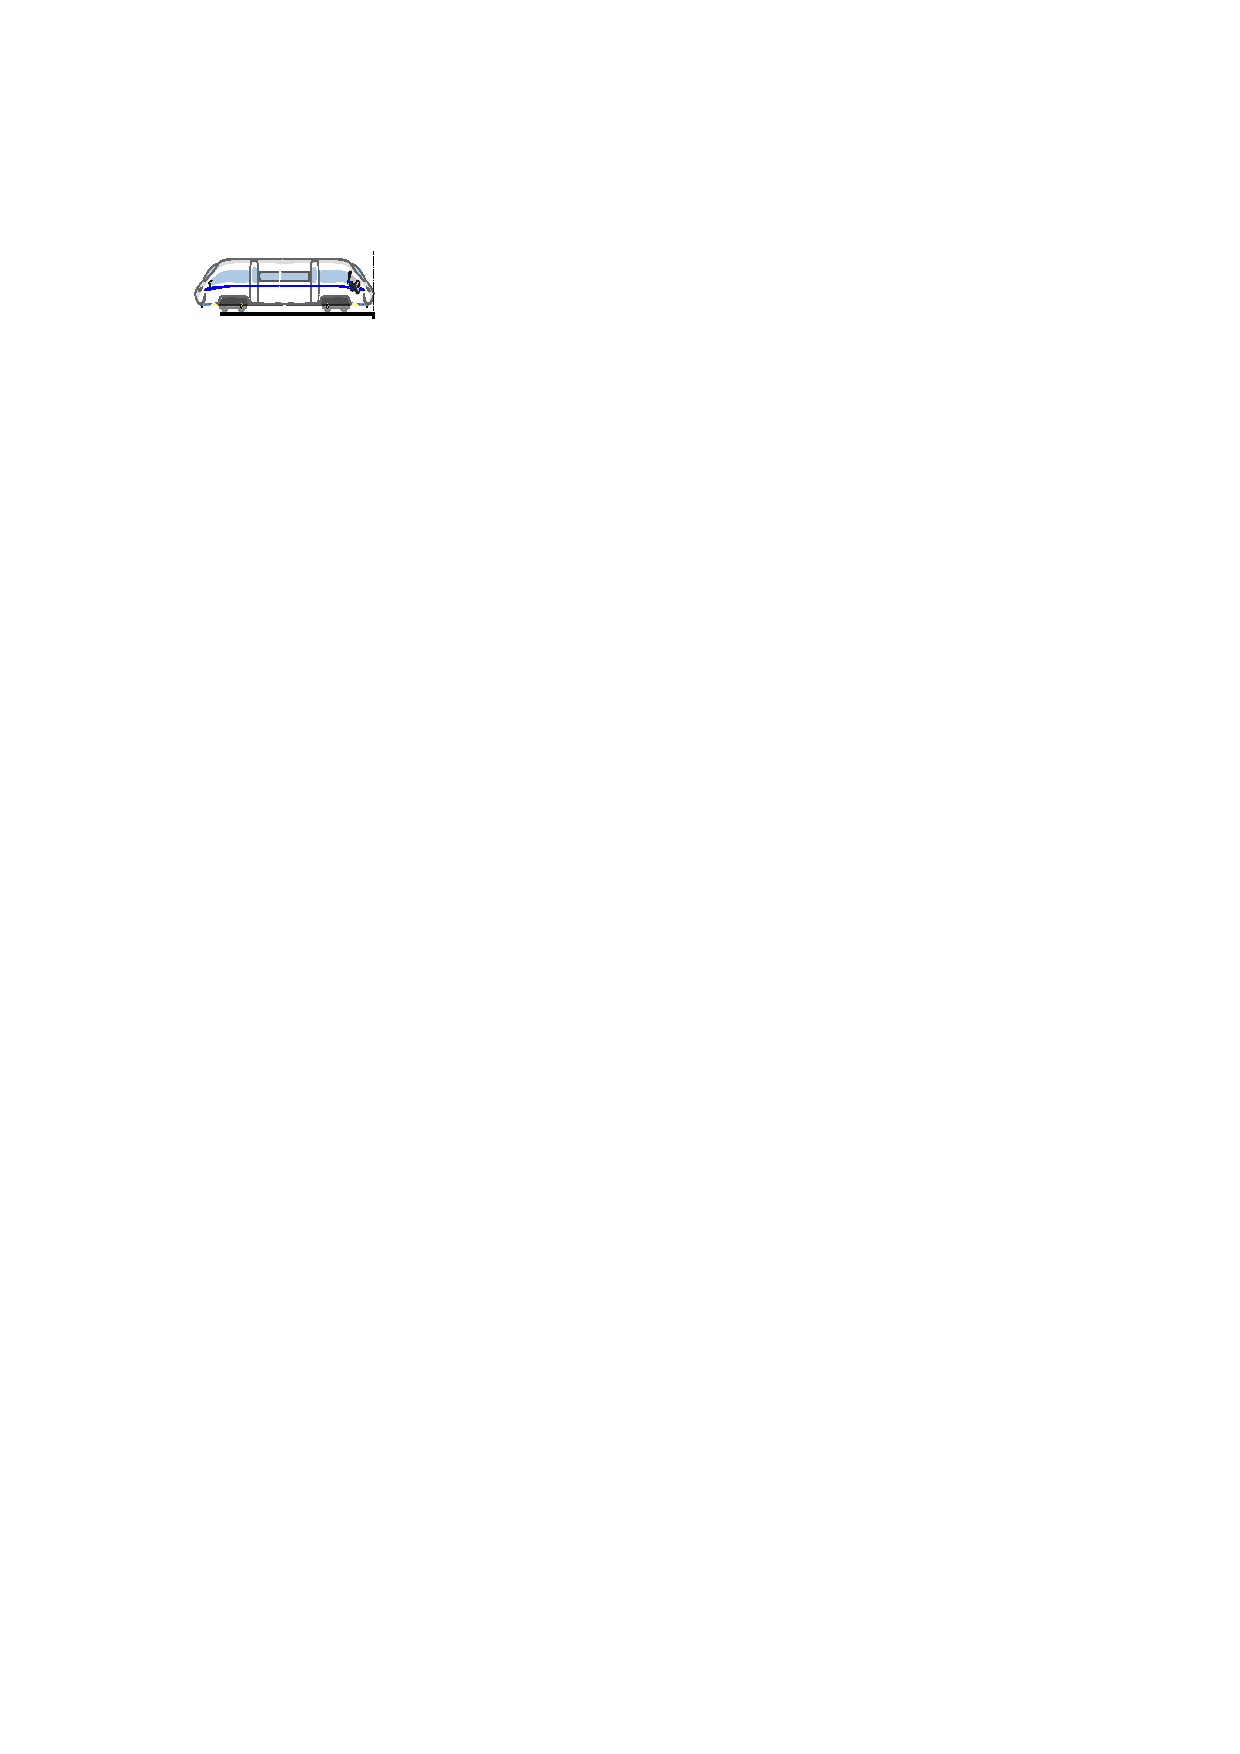
\includegraphics[scale=0.95]{figures/ch2/figure1.pdf}
	\caption{单图示意图}
	\label{fig:ch2-f1}
\end{figure}




\begin{figure}[!htb]
	\centering
	% 第一个子图环境，0.45\textwidth 控制子图占用的宽度比例
	\begin{subfigure}[b]{0.45\textwidth}
		\centering
		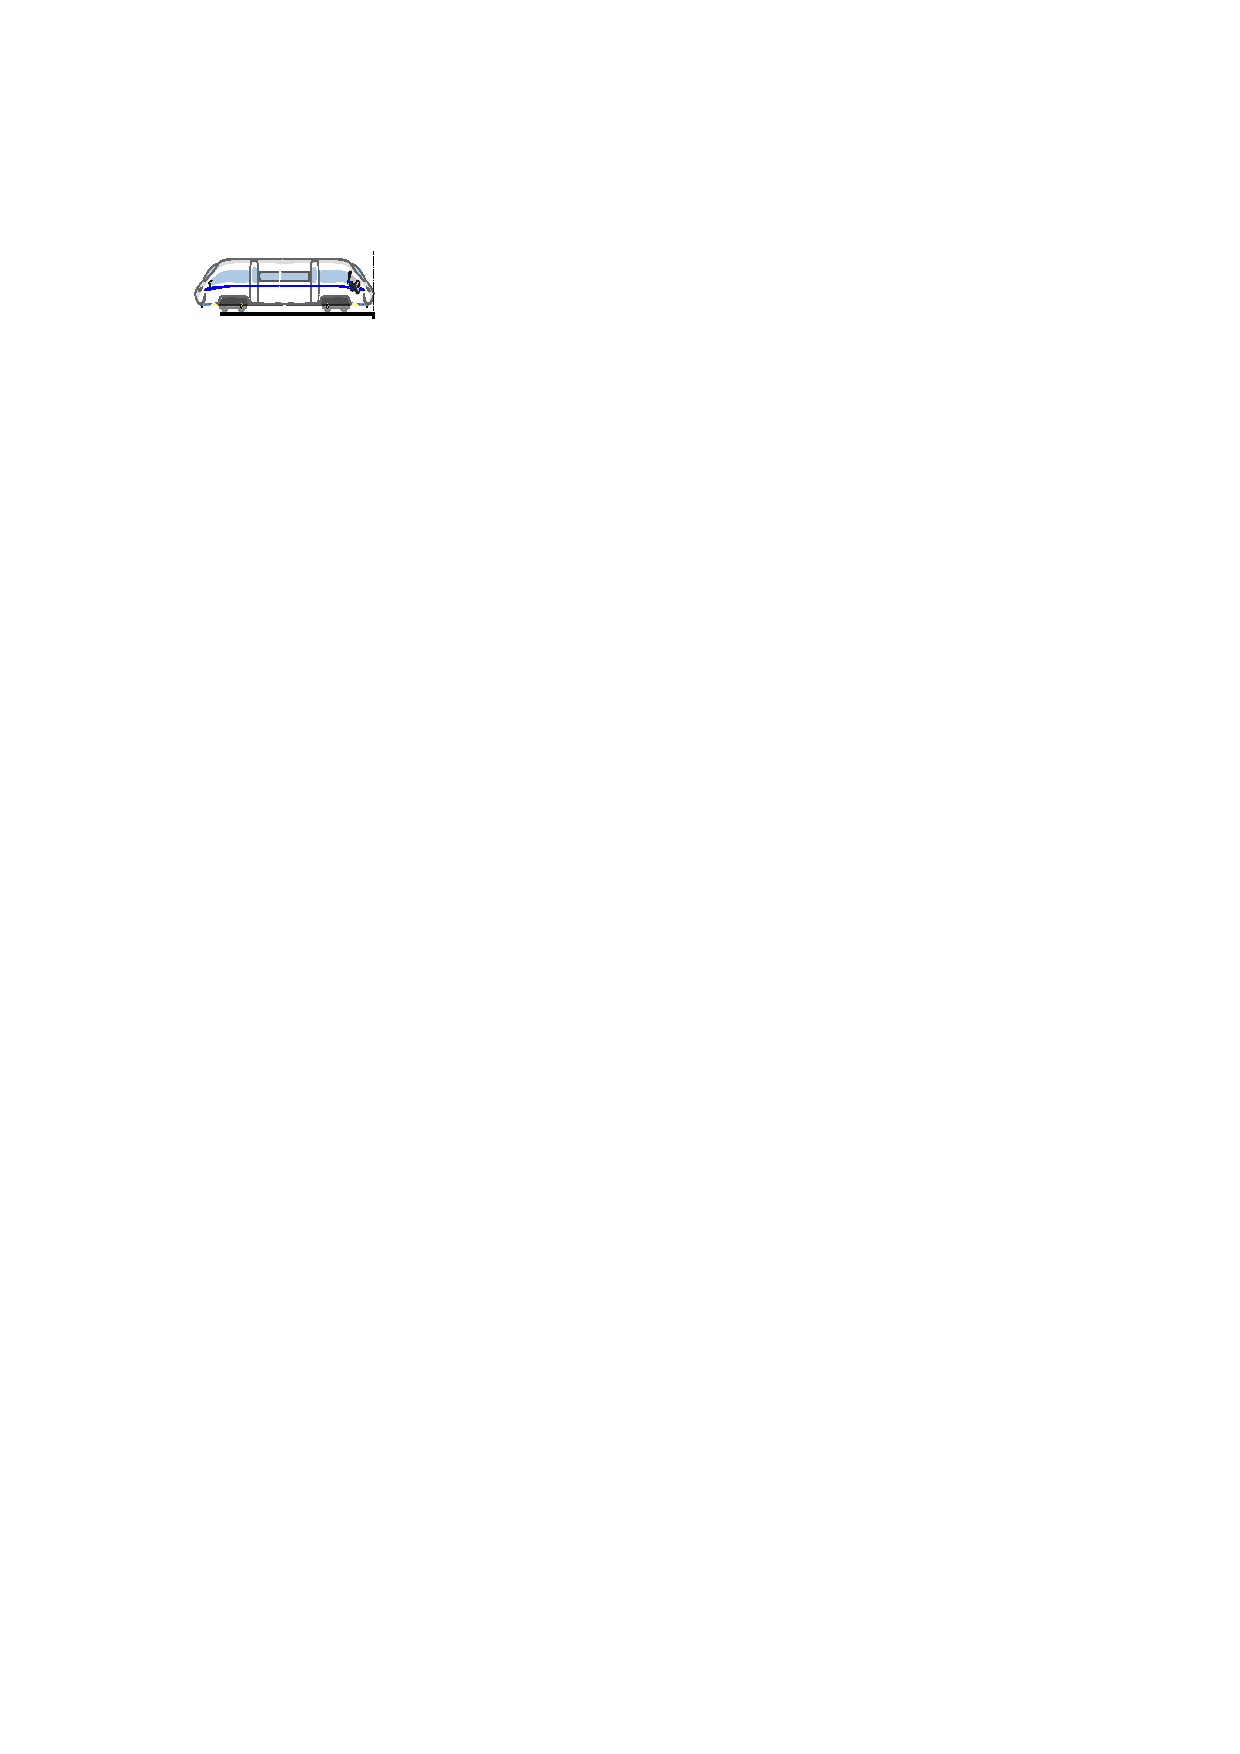
\includegraphics[scale=1]{figures/ch2/figure1.pdf}
		% 在 subcaption 中，直接用 \\ 换行就可以实现双语标题，不需要改计数器！
		\caption{子图1} 
		\label{fig:ch2-sub1}
	\end{subfigure}
	\hspace{5pt} % 子图间距，也可以用 \hfill 让它们自动靠两边对齐
	% 第二个子图环境
	\begin{subfigure}[b]{0.45\textwidth}
		\centering
		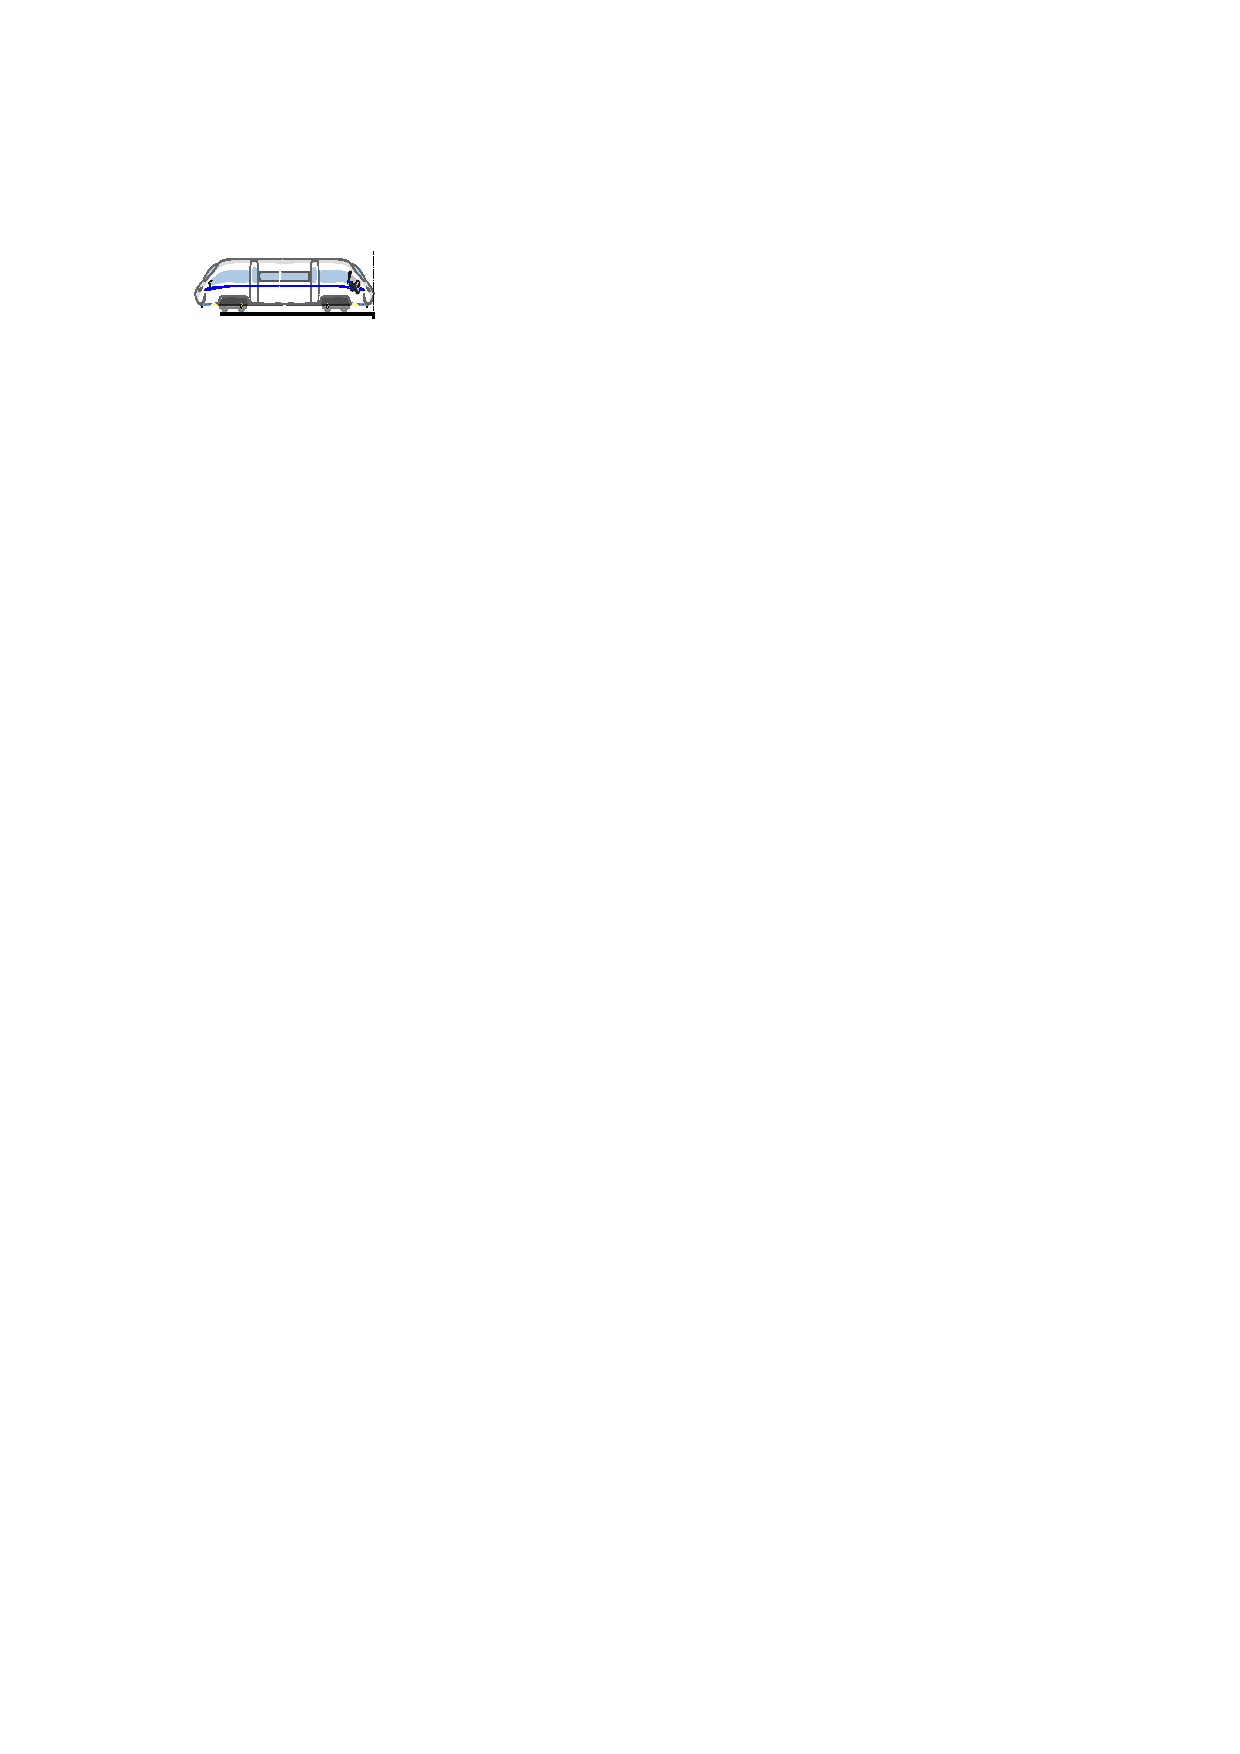
\includegraphics[scale=1]{figures/ch2/figure1.pdf}
		\caption{子图2}
		\label{fig:ch2-sub2}
	\end{subfigure}

        % 第三个子图环境
	\begin{subfigure}[b]{0.45\textwidth}
		\centering
		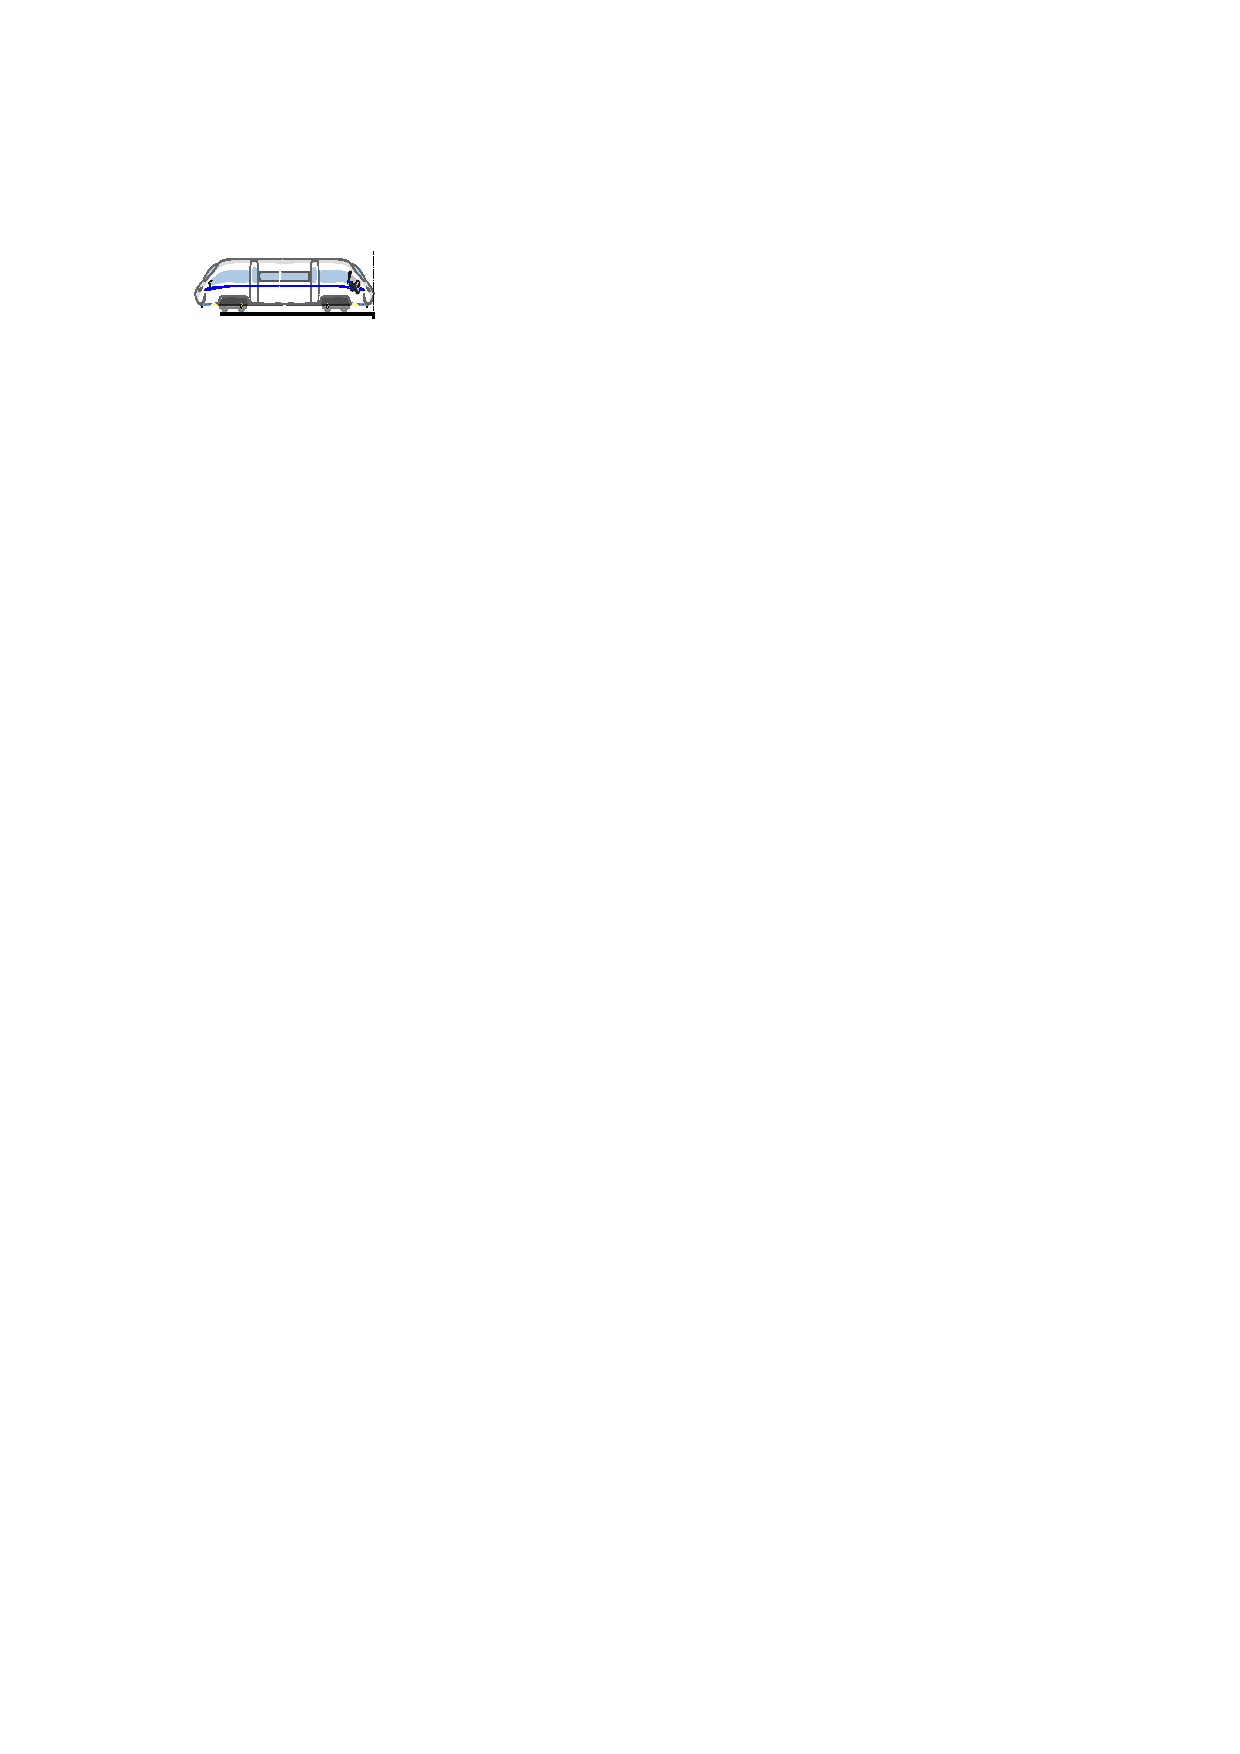
\includegraphics[scale=1]{figures/ch2/figure1.pdf}
		% 在 subcaption 中，直接用 \\ 换行就可以实现双语标题，不需要改计数器！
		\caption{子图3} 
		\label{fig:ch2-sub3}
	\end{subfigure}
	\hspace{5pt} % 子图间距，也可以用 \hfill 让它们自动靠两边对齐
	% 第四个子图环境
	\begin{subfigure}[b]{0.45\textwidth}
		\centering
		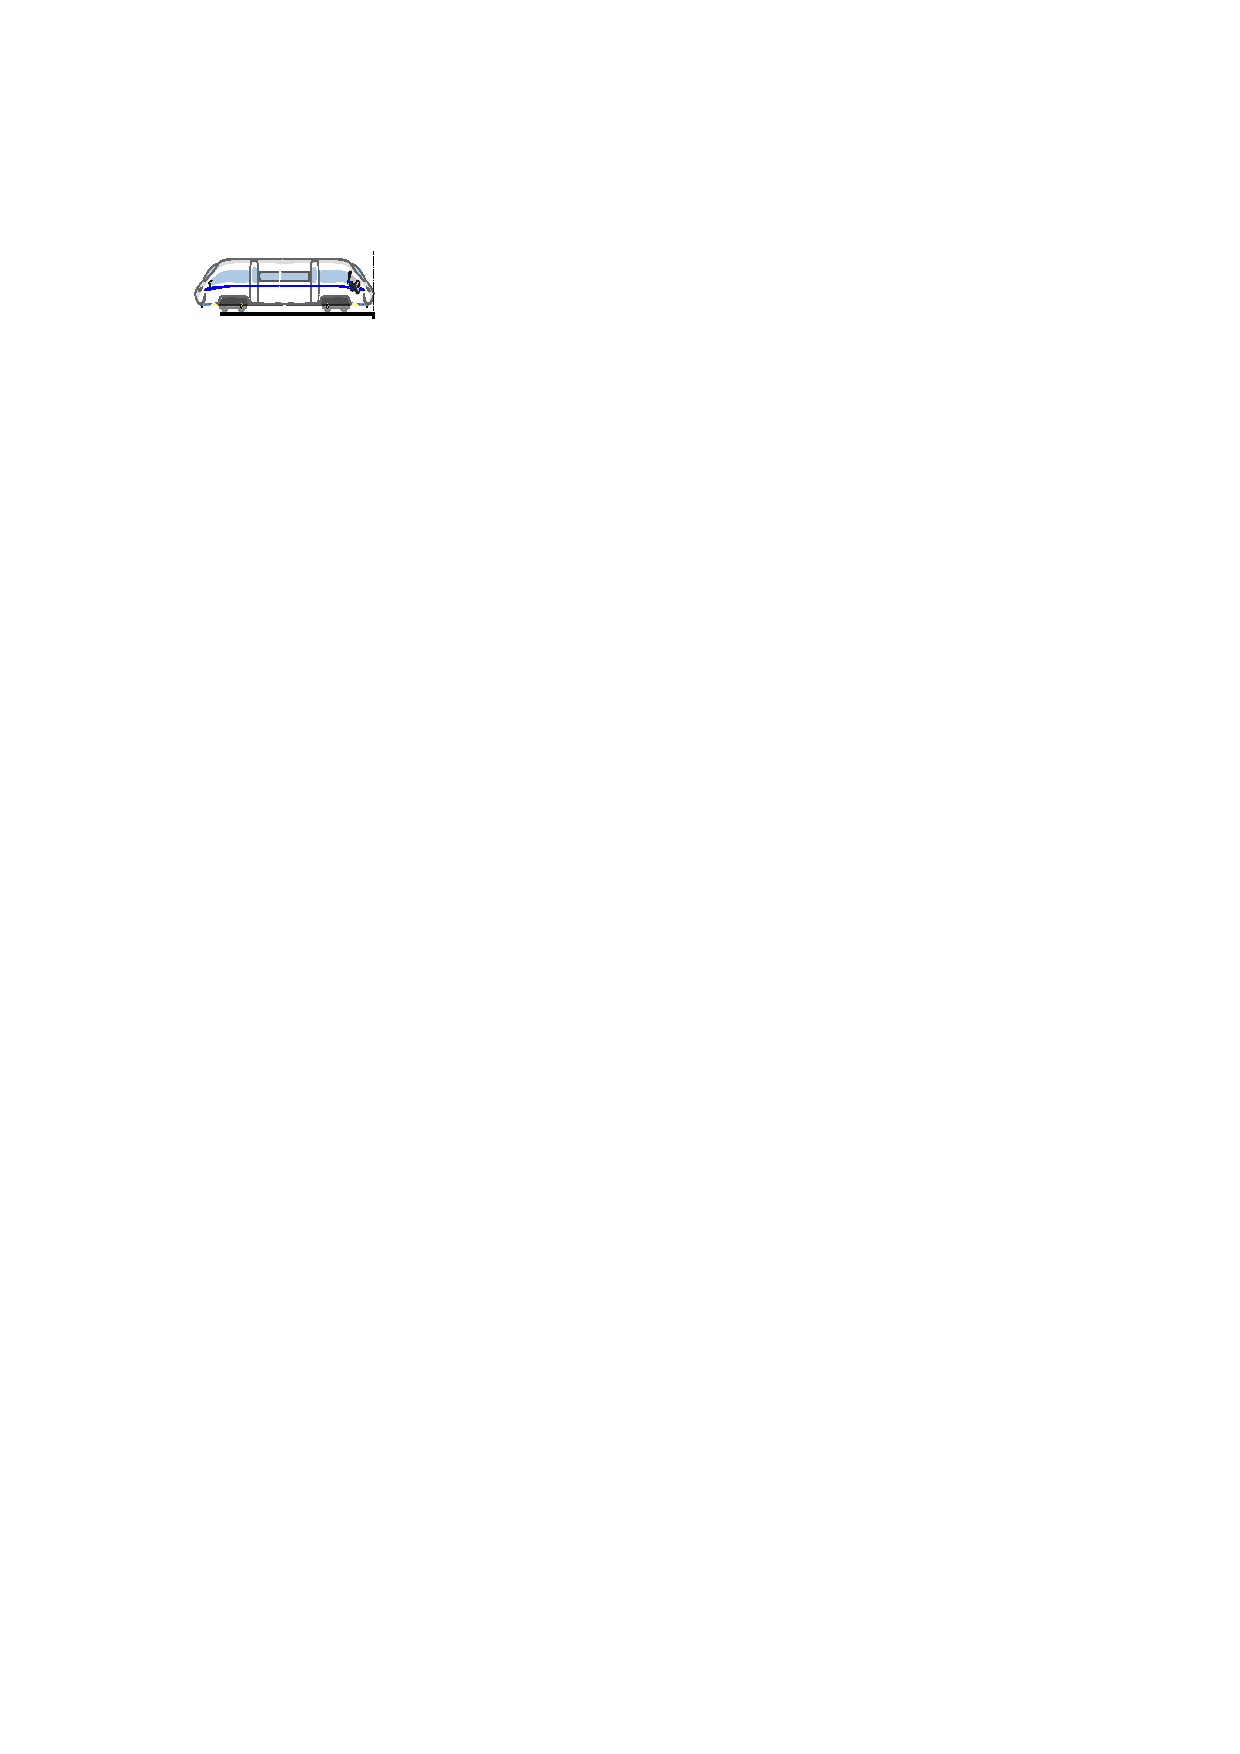
\includegraphics[scale=1]{figures/ch2/figure1.pdf}
		\caption{子图4}
		\label{fig:ch2-sub4}
	\end{subfigure}
	\caption{多图并列示意图}
	\label{fig:ch2-f2}
\end{figure}




\section{表格}

表题置于表的上方，居中。表格的编排建议采用国际通行的三线表，不加左、右边框线。表中文字用宋体（中文）或Times New Roman字体（英文）。

\textbf{带脚注的三线表}：如表\ref{tab:ch2_res1}所示，标题中写不下的内容可放至脚注，此时使用threeparttable包来实现。如果表格超出页面边距或内容太过拥挤，可以使用\textbackslash tabcolsep命令来调节列间距。

\textbf{巨型表格}：表格过大且无法拆分成多个表格时，可以使用sidewaystable旋转表格独占一页，本模板已添加旋转包，只需将\textbackslash begin\{table\}和\textbackslash end\{table\}命令中的table换为sidewaystable即可。如表\ref{tab:ch2_res3}所示。


\begin{table}[!htb]
	\centering
	\small %字体大小
	%\setlength\tabcolsep{3.3pt} %调整列间距
	\caption{性能对比。}
	\begin{threeparttable}
		\begin{tabular}{c|ccc|ccc}
			\toprule
			\multirow{2}{*}{模型} &  & 数据集1 &  &  & 数据集2&  \\
			& MAE & RMSE & MAPE(\%) & MAE & RMSE & MAPE(\%) \\
			\midrule
			
			SVR & 46.46 & 92.97 & 83.40 & 11.10 & 19.84 & 91.96  \\
			LSTM & \textbf{36.20 $\pm$0.17} & \textbf{66.26 $\pm$0.80} & \textbf{40.42 $\pm$0.86} & \textbf{6.70 $\pm$0.02} & \textbf{11.36 $\pm$0.04} & \textbf{74.01 $\pm$1.26}  \\
			\bottomrule
		\end{tabular}
		\begin{tablenotes}
			\footnotesize
			\item[*] 粗体代表所有基准模型中的最佳的性能。
		\end{tablenotes}
	\end{threeparttable}
	\label{tab:ch2_res1}
\end{table}



% 独占一页的表格样例
\begin{sidewaystable}[!htp]
	%\small %字体大小
	\setlength\tabcolsep{20pt} %调整列间距
	\caption{性能对比}
	\begin{threeparttable}
		\begin{tabular}{c|ccc|ccc}
			\toprule
			\multirow{2}{*}{模型} &  & 数据集1 &  &  & 数据集2&  \\
			& MAE & RMSE & MAPE(\%) & MAE & RMSE & MAPE(\%) \\
			\midrule
			
			SVR & 46.46 & 92.97 & 83.40 & 11.10 & 19.84 & 91.96  \\
			LSTM & 36.20 $\pm$0.17 & 66.26 $\pm$0.80 & 40.42 $\pm$0.86 & 6.70 $\pm$0.02 & 11.36 $\pm$0.04 & 74.01 $\pm$1.26  \\
			LSTM & 36.20 $\pm$0.17 & 66.26 $\pm$0.80 & 40.42 $\pm$0.86 & 6.70 $\pm$0.02 & 11.36 $\pm$0.04 & 74.01 $\pm$1.26  \\
			LSTM & 36.20 $\pm$0.17 & 66.26 $\pm$0.80 & 40.42 $\pm$0.86 & 6.70 $\pm$0.02 & 11.36 $\pm$0.04 & 74.01 $\pm$1.26  \\
			LSTM & 36.20 $\pm$0.17 & 66.26 $\pm$0.80 & 40.42 $\pm$0.86 & 6.70 $\pm$0.02 & 11.36 $\pm$0.04 & 74.01 $\pm$1.26  \\
			LSTM & 36.20 $\pm$0.17 & 66.26 $\pm$0.80 & 40.42 $\pm$0.86 & 6.70 $\pm$0.02 & 11.36 $\pm$0.04 & 74.01 $\pm$1.26  \\
			LSTM & 36.20 $\pm$0.17 & 66.26 $\pm$0.80 & 40.42 $\pm$0.86 & 6.70 $\pm$0.02 & 11.36 $\pm$0.04 & 74.01 $\pm$1.26  \\
			LSTM & 36.20 $\pm$0.17 & 66.26 $\pm$0.80 & 40.42 $\pm$0.86 & 6.70 $\pm$0.02 & 11.36 $\pm$0.04 & 74.01 $\pm$1.26  \\
			LSTM & 36.20 $\pm$0.17 & 66.26 $\pm$0.80 & 40.42 $\pm$0.86 & 6.70 $\pm$0.02 & 11.36 $\pm$0.04 & 74.01 $\pm$1.26  \\
			LSTM & 36.20 $\pm$0.17 & 66.26 $\pm$0.80 & 40.42 $\pm$0.86 & 6.70 $\pm$0.02 & 11.36 $\pm$0.04 & 74.01 $\pm$1.26  \\
			LSTM & 36.20 $\pm$0.17 & 66.26 $\pm$0.80 & 40.42 $\pm$0.86 & 6.70 $\pm$0.02 & 11.36 $\pm$0.04 & 74.01 $\pm$1.26  \\
			LSTM & 36.20 $\pm$0.17 & 66.26 $\pm$0.80 & 40.42 $\pm$0.86 & 6.70 $\pm$0.02 & 11.36 $\pm$0.04 & 74.01 $\pm$1.26  \\		
			LSTM & 36.20 $\pm$0.17 & 66.26 $\pm$0.80 & 40.42 $\pm$0.86 & 6.70 $\pm$0.02 & 11.36 $\pm$0.04 & 74.01 $\pm$1.26  \\
			LSTM & 36.20 $\pm$0.17 & 66.26 $\pm$0.80 & 40.42 $\pm$0.86 & 6.70 $\pm$0.02 & 11.36 $\pm$0.04 & 74.01 $\pm$1.26  \\
			LSTM & 36.20 $\pm$0.17 & 66.26 $\pm$0.80 & 40.42 $\pm$0.86 & 6.70 $\pm$0.02 & 11.36 $\pm$0.04 & 74.01 $\pm$1.26  \\
			LSTM & 36.20 $\pm$0.17 & 66.26 $\pm$0.80 & 40.42 $\pm$0.86 & 6.70 $\pm$0.02 & 11.36 $\pm$0.04 & 74.01 $\pm$1.26  \\
			LSTM & \textbf{36.20 $\pm$0.17} & \textbf{66.26 $\pm$0.80} & \textbf{40.42 $\pm$0.86} & \textbf{6.70 $\pm$0.02} & \textbf{11.36 $\pm$0.04} & \textbf{74.01 $\pm$1.26}  \\
			\bottomrule
		\end{tabular}
		\begin{tablenotes}
			\footnotesize
			\item[*] 粗体代表所有基准模型中的最佳的性能。
		\end{tablenotes}
	\end{threeparttable}
	\label{tab:ch2_res3}
\end{sidewaystable}


